\documentclass[12pt, a4paper]{article}
\usepackage{graphicx}
\usepackage{geometry}
\geometry{a4paper, margin=1in}
\usepackage{tabularx}
\usepackage{booktabs}
\usepackage{array}
\usepackage{hyperref}
\usepackage{fancyhdr}
\usepackage{float}


\pagestyle{fancy}
\fancyhf{}
\fancyhead[L]{Gym Membership Management System}
\fancyhead[R]{Group 6}
\fancyfoot[C]{\thepage}
\renewcommand{\headrulewidth}{0.4pt}

\begin{document}

% --- TITLE PAGE ---
\begin{titlepage}
    \centering
    \linespread{1.5}\selectfont % Maintains the 1.5 line spacing
    
    
\includegraphics[width=0.4\textwidth]{umt_logo.png}\par
    \vspace{0.5cm}
    
    \textbf{FACULTY OF COMPUTER SCIENCE AND MATHEMATICS}\par
    BACHELOR OF COMPUTER SCIENCE (SOFTWARE ENGINEERING) WITH HONORS\par
    \vspace{0.5cm}
    
    CSE3023 WEB-BASED APPLICATION DEVELOPMENT\\
    SEMESTER II 2025/2026\par
    \vspace{0.5cm}
    
    GROUP NUMBER:\\
    \textbf{6}\par
    \vspace{0.5cm}
    
    \textbf{GYM MEMBERSHIP MANAGEMENT SYSTEM}\par
    \vspace{0.8cm}
    
    PREPARED BY:\par
    \begin{table}[h!]
        \centering
        \renewcommand{\arraystretch}{1.2} % Adjusts the table row height slightly
        \begin{tabular}{|c|c|}
            \hline
            NAME & MATRIC NO. \\ \hline
            NUR ADLYNN SYAKIRAH BINTI NOR KHAIRUL ANUAR & S76245 \\ \hline
            NURBATRISYIA ALIZA BINTI ALIAS & S75516 \\ \hline
            WAN NUR SYAFIQAH IZANI BINTI WAN HIZHAN & S75776 \\ \hline
        \end{tabular}
    \end{table}
    
    \vfill % This automatically calculates the remaining space and pushes the text below to the bottom margin
    
    PREPARED FOR:\\
    TS. DR. WAN NURAL JAWAHIR BINTI HJ WAN YUSSOF\par
    \vspace{0.8cm}
    
    SUBMISSION DATE:\\
    05\textsuperscript{TH} MAY 2026\par
    \vspace{0.5cm}
\end{titlepage}

% --- TABLE OF CONTENTS ---
\tableofcontents
\newpage

\listoftables
\listoffigures
\newpage

% --- SECTION 1.0 ---
\section{Introduction}

\subsection{Project Overview}
The Gym Membership Management System is a web-based application developed using Java-based MVC architecture to support the daily operations of a gym environment. 
The system is designed to replace traditional manual methods such as spreadsheets and paper records, which are often slow, inconsistent, and prone to human error.
In many gym settings, managing member attendance, class bookings, and payment records can become disorganised when handled separately.
Information is usually scattered across different files or systems, making it difficult for staff to track updates or retrieve accurate records quickly.
This situation can lead to confusion in scheduling, mistakes in attendance tracking, and delays in processing payments. 

To address these issues, this system provides a centralised platform where gym operations can be managed more efficiently.
It focuses on three main functional areas: attendance and check-in management, class booking and scheduling, and billing and payment management.
Each of these modules allows users to perform basic data management operations such as adding new records, viewing existing information, updating details, and removing outdated entries.

The system is developed using the Model-View-Controller (MVC) architecture to ensure proper separation of concerns.
The Model layer handles the data structure and business logic, such as storing member details, bookings, and payment information.
The View layer is responsible for the user interface, implemented using JSP, HTML, and CSS, allowing users to interact with the system in a structured and user-friendly way.
The Controller layer, implemented using Servlets, processes user requests and manages communication between the interface and the underlying data.
By structuring the system in this way, it becomes easier to maintain and expand in the future. 
Changes to the interface, business logic, or data structure can be made independently without affecting the entire system.
Overall, this project aims to improve the efficiency of gym management operations while providing a more organised and reliable way of handling member-related activities.

\subsection{Problem Statement}
Existing gym management practices often rely on manual processes or fragmented systems such as spreadsheets, which are inefficient and difficult to maintain. 
These approaches increase the risk of data inconsistency, human error, and loss of important information, particularly in managing memberships, attendance, class schedules, and payments. 
The absence of a centralized system limits the ability of administrators to monitor operations in real time, generate accurate reports, and ensure proper coordination between members and trainers. 
As a result, tasks such as tracking attendance, scheduling classes, and managing billing become time-consuming and prone to errors. 
Furthermore, members and trainers have limited access to timely and accurate information, leading to poor user experience and reduced operational efficiency.
Therefore, a structured and integrated web-based system is required to address these limitations and improve the overall management of gym services.

% --- SECTION 2.0 ---
\section{Functional Module Allocation}

\subsection{Module Distribution}

\begin{table}[h!]
    \centering
    \caption{Project Module Allocation and Member Responsibilities}
    \renewcommand{\arraystretch}{1.2}
    \begin{tabularx}{\textwidth}{|p{5cm}|p{4cm}|X|}
        \hline
        \textbf{Member} & \textbf{Module} & \textbf{Description} \\ \hline
        Nur Adlynn Syakirah Binti Nor Khairul Anuar (Leader) 
        & Attendance and Check-in Management 
        & Manages member attendance records, including check-in, check-out, and attendance tracking for gym activities and classes. Supports full CRUD operations. \\ \hline
        
        Nurbatrisyia Aliza Binti Alias 
        & Billing and Payment Management 
        & Manages membership payments, billing records, and transaction history. Includes payment creation, updates, deletion, and viewing of payment status. Supports full CRUD operations. \\ \hline
        
        Wan Nur Syafiqah Izani Binti Wan Hizhan 
        & Class Booking and Scheduling Management 
        & Handles gym class schedules and booking activities. Members can book or cancel classes, while trainers and admin manage session schedules. Supports full CRUD operations. \\ \hline
    \end{tabularx}
\end{table}

\subsection{Mandatory Requirement}

\subsubsection{Manage Attendance and Check-in}
This module is responsible for managing attendance records of gym members. 
It allows members to check in and check out of the gym, while trainers can record attendance for scheduled classes. 
The admin can monitor attendance reports and ensure data accuracy. 
The module supports full CRUD operations where new attendance records are created during check-in or class attendance marking, existing records can be retrieved for reporting purposes, updates can be made to correct attendance details, and incorrect or duplicate records can be deleted by the admin. 

\subsubsection{Manage Booking and Schedule} 
This module is responsible for managing bookings and schedules management for gym classes and training sessions. 
Members are able to create bookings by selecting available time slots based on existing schedules. 
Administrators and trainers are responsible for creating, updating and managing schedules, including session details such as date, time, trainer assignment, and capacity limits. 
The system allow member to view available sessions and their booking status in real time. 
Booking may be updated when members reschedule sessions, while cancellations or deletions are permitted based on system rules and availability constraints. 
This ensures efficient scheduling and prevents conflicts such as double booking or overcapacity. 

\subsubsection{Manage Billing and Payment} 
This module is used to manage all payment-related processes in the gym system. 
It records payments made by members and keeps track of their billing status. 
Admins are responsible for handling payment records, such as creating new transactions, updating payment status, and maintaining proper billing history. 
Members can also view their payment history to check what they have paid and whether their payments are up to date. 
This helps make the financial process more transparent and easier to track. 
Like the other modules, this one also supports full CRUD operations, where payment records can be created, retrieved, updated, and deleted when necessary. 

% --- SECTION 3.0 ---
\section{Use Case Diagram} 

\begin{figure}[h!]
    \centering
    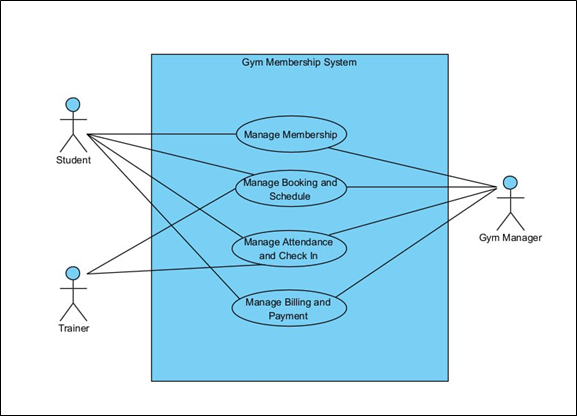
\includegraphics[width=0.8\textwidth]{use_case_diagram.png}
    \caption{Use Case Diagram for Gym Membership Management System}
\end{figure}

% Use Case 1 Table
\begin{table}[H]
    \centering
    \caption{Use Case 1: Manage Membership}
    \renewcommand{\arraystretch}{1.3}
    \begin{tabularx}{\textwidth}{X}
        \hline
        \textbf{Use Case Name:} Manage Membership \hfill \textbf{ID:} UC1 \hfill \textbf{Importance Level:} High \\
        \hline
        \textbf{Primary Actor:} Student, Gym Manager \hfill \textbf{Use Case Type:} Primary, Essential \\
        \textbf{Stakeholder and Interests:} \\
        Student - wants their membership details to be accurate and easily accessible, including status and expiry date. \\
        Gym Manager - needs to manage member records efficiently and ensure all membership information is up to date. \\
        \textbf{Brief Description:} This use case describes how membership information is handled within the system. The gym manager is responsible for creating, updating, and maintaining member records, while members can view their own membership details. The system keeps track of membership status and expiry dates to ensure that only active students can access gym services. \\
        \textbf{Trigger:} External: A new member registers, or an existing membership needs to be updated or renewed. \\
        \textbf{Type:} External \\
        \textbf{Relationship:} \\
        Associated Classes: Student, Membership \\
        \textbf{Normal Flow of Events:} \\
        1. The Gym Manager accesses the membership management module. \\
        2. The Gym Manager registers a new member by entering personal details such as name, email, and contact number. \\
        3. The Gym Manager assigns a membership plan (e.g., monthly or yearly) and sets the start and expiry date. \\
        4. The system validates the entered information. \\
        5. The system creates a new member record and stores the membership details with an “Active” status. \\
        6. The Student logs into the system. \\
        7. The Student views their profile and membership information, including status and expiry date. \\
        8. If needed, the Gym Manager updates member details or membership information. \\
        9. When a membership is close to expiry, the Gym Manager renews the membership by updating the expiry date. \\
        10. The system saves all updated information. \\
        \textbf{Sub-Flows:} \\
        Membership Validation: The system checks that all required fields are completed and ensures that the membership dates are valid before saving the record. \\
        \textbf{Alternate/Exceptional Flows:} \\
        4a. Missing or invalid student details; the system displays an error and prevents submission. \\
        \hline
    \end{tabularx}
\end{table}

\newpage

% --- Continuation of Use Case 1 Table ---
\begin{table}[H]
    \centering
    \renewcommand{\arraystretch}{1.3}
    \begin{tabularx}{\textwidth}{X}
        \hline
        7a. Student record not found; the system shows a message indicating that no profile exists. \\
        9a. Renewal is attempted on an inactive or non-existent membership; the system rejects the action. \\
        \hline
    \end{tabularx}
\end{table}

%use case 2
\begin{table}[H]
    \centering
    \caption{Use Case 2: Manage Booking and Schedule}
    \renewcommand{\arraystretch}{1.3} % Controlled spacing for a neat look 
    \small
    \begin{tabularx}{\textwidth}{X}
        \hline
        \textbf{Use Case Name:} Manage Booking \& Schedule \hfill \textbf{ID:} UC2 \hfill \textbf{Importance Level:} High \\
        \hline
        \textbf{Primary Actor:} Student, Trainer, Gym Manager \hfill \textbf{Use Case Type:} Primary, Essential \\
        \textbf{Stakeholder and Interests:} \\
        Student -- wants to reserve slots for classes or training sessions easily. \\
        Trainer -- needs to view and manage their assigned teaching schedule efficiently. \\
        Gym Manager -- needs to create and modify the master schedule to avoid conflicts. \\
        \textbf{Brief Description:} This use case details the process of creating gym schedules and allowing members to book slots within capacity limits. The Gym Manager or Trainer creates schedules, while students can view available sessions and make bookings. \\
        \textbf{Trigger:} External: A student attempts to book a class or an admin adds a new class to the calendar. \\
        \textbf{Type:} External \\
        \textbf{Relationship:} \\
        Associated Classes: Student, Trainer, Schedule, Booking  \\
        \textbf{Normal Flow of Events:} \\
             1. The Gym Manager creates a new class schedule including time, trainer, and capacity.\\
             2. The Student logs into the system and views available time slots on the dashboard.\\
            3. The Student selects a preferred slot and initiates a booking request.\\
            4. The system validates the booking and updates the remaining capacity for that session.\\
            5. The system creates a booking record for the student with a "Confirmed" status.\\
            6. The Trainer views their updated schedule to see the current list of registered students.\\
            7. The Student receives a booking confirmation and can view it in their profile.\\
            8. If necessary, the Gym Manager or Trainer updates the class details or cancels a session.\\
            9. The system saves all updated schedule and booking information.\\
         
        \textbf{Sub-Flows:} \\
        Capacity Check: The system validates that the current booking count is less than the maximum capacity before confirming the reservation. \\
        \textbf{Alternate/Exceptional Flows:} \\
        4a. Class is full; the system notifies the student and suggests alternative time slots. \\
        4b. Double Booking; the system prevents a student from booking two classes at the same time. \\
        \hline
    \end{tabularx}
\end{table}

%Use Case 3
\begin{table}[H]
    \centering
    \caption{Manage Attendance and Check-in}
    \renewcommand{\arraystretch}{1.3} % Matches your preferred compact spacing
    \small
    \begin{tabularx}{\textwidth}{X}
        \hline
        \textbf{Use Case Name:} Manage Attendance \hfill \textbf{ID:} UC3 \hfill \textbf{Importance Level:} High \\
        \hline
        \textbf{Primary Actor:} Student, Trainer, Gym Manager \hfill \textbf{Use Case Type:} Primary, Essential \\
        \textbf{Stakeholder and Interests:} \\
        Student -- wants to record their gym entry and exit accurately to track personal activity. \\
        Trainer -- needs to mark attendance for members attending scheduled classes. \\
        Gym Manager -- needs accurate attendance data to monitor facility usage and generate reports. \\
        \textbf{Brief Description:} This use case describes how the system records student entry (check-in) and exit (check-out), and how trainers or managers manage these records to ensure data accuracy. \\
        \textbf{Trigger:} External: A student arrives at the gym or a trainer begins a scheduled class session. \\
        \textbf{Type:} External \\
        \textbf{Relationship:} \\
        Associated Classes: Student, Trainer, Attendance  \\
        \textbf{Normal Flow of Events:}
    
            1. The Student initiates a check-in at the gym entrance via the system interface.\\
            2. The system validates the student's membership status and records the entry timestamp.\\
            3. For scheduled classes, the Trainer accesses the session and views the list of registered students.\\
            4. The Trainer marks each student as "Present" or "Absent" based on their attendance.\\
            5. The Student initiates a check-out when leaving, and the system records the exit timestamp.\\
            6. The Gym Manager accesses the attendance module to monitor overall activity and ensure data integrity.\\
            7. The system saves all attendance records and updates activity reports.\\
        
        \textbf{Sub-Flows:} \\
        Status Verification: The system automatically checks if the student's membership status is "Active" before permitting a check-in. \\
        \textbf{Alternate/Exceptional Flows:} \\
        2a. Membership is expired; the system denies check-in and prompts the student to renew. \\
        4a. Trainer attempts to mark attendance for a future class; the system disables the marking function until the class starts. \\
        \hline
    \end{tabularx}
\end{table}


% Use Case 4 Table
\begin{table}[H]
    \centering
    \caption{Use Case 4: Manage Billing and Payment}
    \renewcommand{\arraystretch}{1.3}
    \begin{tabularx}{\textwidth}{X}
        \hline
        \textbf{Use Case Name:} Manage Billing and Payment \hfill \textbf{ID:} UC4 \hfill \textbf{Importance Level:} High \\
        \hline
        \textbf{Primary Actor:} Student, Gym Manager \hfill \textbf{Use Case Type:} Primary, Essential \\
        \textbf{Stakeholder and Interests:} \\
        Student - wants to clearly see their payment status and avoid confusion about outstanding fees. \\
        Gym Manager - needs a reliable way to record payments and make sure billing records are accurate and up to date. \\
        \textbf{Brief Description:} This use case explains how payment records are handled in the gym system. The gym manager is responsible for creating and updating billing records, while students can view their payment details and complete payments. The system keeps track of payment status so that both sides can easily monitor whether fees are settled or still pending. \\
        \textbf{Trigger:} External: A gym manager records a payment or a student checks their billing information. \\
        \textbf{Type:} External \\
        \textbf{Relationship:} \\
        Associated Classes: Payment, Student, Membership \\
        \textbf{Normal Flow of Events:} \\
        1. The Gym Manager opens the billing module from the system dashboard. \\
        2. The Gym Manager enters the member ID along with payment details such as amount and membership type (e.g., monthly or yearly). \\
        3. The system checks whether the member exists and whether the entered amount is valid. \\
        4. If everything is correct, the system stores the payment record with a status such as “Pending” or “Paid”. \\
        5. The Student logs into the system and navigates to the payment section. \\
        6. The Student views their payment history and current billing status. \\
        7. If there is an outstanding fee, the Student proceeds to make a payment. \\
        8. The system updates the payment status to “Paid” after the transaction is completed. \\
        9. The Gym Manager can later review all payment records or generate simple reports when needed. \\
        \textbf{Sub-Flows:} \\
        Payment Validation: Before saving any record, the system ensures that the member ID is valid and the payment amount matches the selected membership plan. This helps avoid incorrect billing entries. \\
        \textbf{Alternate/Exceptional Flows:} \\
        3a. The student ID does not exist; the system displays an error and stops the process. \\
        7a. The payment attempt fails; the system notifies the student and allows another attempt. \\
        \hline
    \end{tabularx}
\end{table}

% --- Continuation of Use Case 4 Table ---
\begin{table}[H]
    \centering
    \renewcommand{\arraystretch}{1.3}
    \begin{tabularx}{\textwidth}{X}
        \hline
        6a. No payment record is found; the system shows a message indicating that no billing data is available. \\
        \hline
    \end{tabularx}
\end{table}

% --- SECTION 4.0 ---
\section{Class Diagram} 

\begin{figure}[H]
    \centering
    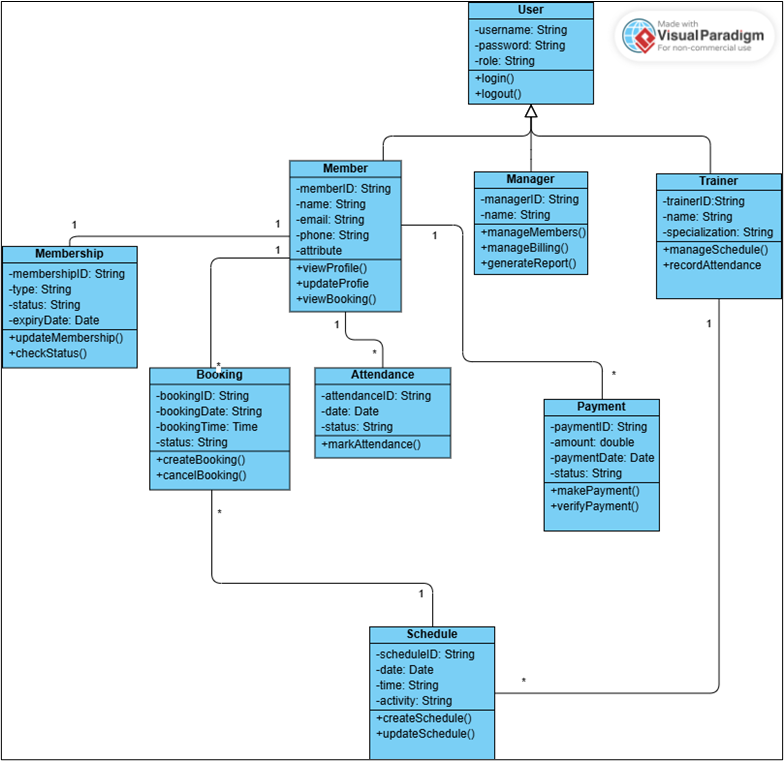
\includegraphics[width=1\textwidth]{class_diagram.png}
    \caption{Class Diagram for Gym Membership Management System}
\end{figure}

The class diagram for the Gym Membership System represents the overall structure of the system, showing the main classes, their attributes, operations, and the relationships between them. 
The system is built around a general User class, which acts as a parent (superclass) for three specialized roles which are Member, Manager, and Trainer. 
The User class contains common attributes such as username, password, and role, along with basic operations like login() and logout(), which are shared by all users in the system. 

The Member class extends the User class and represents gym customers who register for membership. 
Each member has personal details such as memberID, name, email, and phone number. 
Members can view and update their profile and view booking information. 
Each member is associated with a Membership record, which stores details like membershipID, type, status, and expiry date. 
The MembershipID class also includes operations to update membership information and check membership status. 
Members are also linked to Booking Attendance, and Payment classess.
A member can make multiple bookings for gym sessions, where each booking includes details such as bookingID, date, time, and status, and supports operations like createBooking() and cancelBooking(). 
Attendance record track member participation in activities, storing attendanceID, date, and status, with markAttendance() function. 
Payment records manage financial transactions, including paymentID, amount, payment date, and status, with operations such as makePayment() and verifyPayment(). 

The Trainer class represents gym trainers who manage workout schedules and record attendance. 
Trainers have attributes like trainerID, name, and specialization, and can manage schedules and record member attendance. 
The Schedule class is associated with trainers and bookings, containing scheduleID, date, time, and activity details, with operations to create and update schedules. 
Meanwhile, the Manager class handles administrative functions such as managing members, handling billing, and generating reports, making it responsible for overseeing the overall system of operations. 

In conclusion, the system is structured to separate responsibilities between users while clearly maintaining strong relationships between membership, booking, attendance, payment, and scheduling functions, ensuring smooth management of gym operations. 

\end{document}